\section{Eksperimenti i analiza rezultata}

U ovom poglavlju detaljno se opisuje eksperimentalni postav, provedba eksperimenata te analiza i interpretacija dobivenih rezultata. Cilj je bio empirijski validirati predloženi hibridni model i usporediti ga s drugim pristupima.

\subsection{Postavke okruženja i testni podaci}

Svi eksperimenti provedeni su u programskom okruženju Python (verzija 3.x) na standardnom osobnom računalu. Za potrebe istraživanja generiran je sintetički skup podataka koji oponaša realističan projektni portfelj. Skup se sastoji od 50 jedinstvenih projektnih aktivnosti (\texttt{NUM\_ACTIVITIES = 50}). Za svaku aktivnost definirani su sljedeći parametri unutar zadanih raspona:

\begin{itemize}
  \item \textbf{Trošak (cost):} Slučajna cjelobrojna vrijednost između 50 i 200.
  \item \textbf{ROI (roi):} Slučajna decimalna vrijednost između 1.0 i 3.0.
  \item \textbf{Procjene trajanja:}
  \begin{itemize}
    \item Optimistično: između 5 i 10 dana.
    \item Najvjerojatnije: između 10 i 20 dana.
    \item Pesimistično: između 20 i 40 dana.
  \end{itemize}
\end{itemize}

Ukupni raspoloživi budžet za portfelj postavljen je na 1000 jedinica (\texttt{BUDGET = 1000}).

\subsection{Eksperimentalni dizajn}

Kako bi se osigurala metodološka ispravnost i izbjegli proizvoljni zaključci, istraživanje je provedeno kroz dvofazni eksperimentalni proces:

\begin{itemize}
  \item \textbf{Faza 1:} Analiza i kalibracija genetskog algoritma. U prvoj fazi provedena je detaljna ablacijska studija kako bi se utvrdilo koji parametri genetskog algoritma daju najkvalitetnija i najstabilnija rješenja za zadani tip problema. Cilj je bio pronaći ``šampionsku'' konfiguraciju GA.
  
  \item \textbf{Faza 2:} Usporedna analiza optimizacijskih modela. U drugoj fazi, ``šampionska'' konfiguracija GA, dobivena u prvoj fazi, korištena je za provođenje konačne usporedbe triju različitih optimizacijskih scenarija i evaluaciju glavne hipoteze rada.
\end{itemize}

\subsection{Eksperiment 1: Analiza parametara i kalibracija genetskog algoritma}

\textbf{Cilj:} Empirijski provjeriti utjecaj osnovnih genetskih operatora i parametara na performanse algoritma te odabrati optimalnu konfiguraciju za daljnje testiranje.

\textbf{Metodologija:} Provedena je ablacijska studija s pet različitih konfiguracija, gdje je svaka pokrenuta 10 puta (\texttt{RUNS = 10}) radi statističke pouzdanosti. Testirane konfiguracije su bile: \emph{Standardni GA}, \emph{Bez mutacije}, \emph{Bez križanja}, \emph{Više generacija} i \emph{Veća populacija}.

\textbf{Rezultati i diskusija:} Rezultati ablacijske studije prikazani su u Tablici~\ref{tab:ga_ablation} te pružaju uvid u dinamiku ponašanja genetskog algoritma.

\begin{table}[H]
\centering
\caption{Rezultati ablacijske studije za parametre GA}
\label{tab:ga_ablation}
\begin{tabular}{|l|c|c|c|c|}
\hline
\textbf{Postavka} & \textbf{ROI\_mean} & \textbf{ROI\_std} & \textbf{Trajanje\_mean} & \textbf{Trajanje\_std} \\
\hline
Standardni GA     & 28.985  & 1.543  & 199.216  & 10.691 \\
Bez mutacije      & 27.627  & 1.581  & 193.497  & 11.364 \\
Bez križanja      & 25.884  & 1.865  & 191.514  & 9.174  \\
Više generacija   & 31.183  & 0.928  & 205.026  & 13.649 \\
Veća populacija   & \textbf{31.683}  & \textbf{0.720}  & \textbf{213.694}  & \textbf{5.574}  \\
\hline
\end{tabular}
\end{table}

Analiza rezultata potvrđuje obje početne hipoteze. 

Prvo, vidljivo je da su genetski operatori križanje i mutacija esencijalni. Uklanjanje križanja drastično smanjuje performanse (\texttt{ROI\_mean} pada na 25.88), što ukazuje da je rekombinacija dobrih rješenja ključan mehanizam pretrage. Uklanjanje mutacije također smanjuje performanse, potvrđujući njezinu ulogu u održavanju genetske raznolikosti i izbjegavanju prerane konvergencije.

Drugo, povećanje računalnih resursa ima direktan pozitivan utjecaj. I \emph{Više generacija} i \emph{Veća populacija} značajno su nadmašile standardnu konfiguraciju. Konfiguracija \emph{Veća populacija} pokazala se superiornom, ostvarivši najviši prosječni ROI (31.683) uz najnižu standardnu devijaciju (0.720). To ukazuje da za ovaj problem veća početna raznolikost rješenja (širina pretrage) donosi bolje rezultate od dužeg trajanja evolucije (dubina pretrage).

Zanimljivo je primijetiti da konfiguracije s najvišim ROI-em ujedno rezultiraju i najdužim prosječnim trajanjem projekta. To sugerira da su najprofitabilnije aktivnosti inherentno povezane s većim vremenskim ulaganjem, što stvara prirodni kompromis (\emph{trade-off}) između profita i rizika trajanja. Upravljanje tim kompromisom bit će predmet analize u sljedećem eksperimentu.


\begin{figure}[H]
    \centering
    \begin{subfigure}[b]{0.48\textwidth}
        \centering
        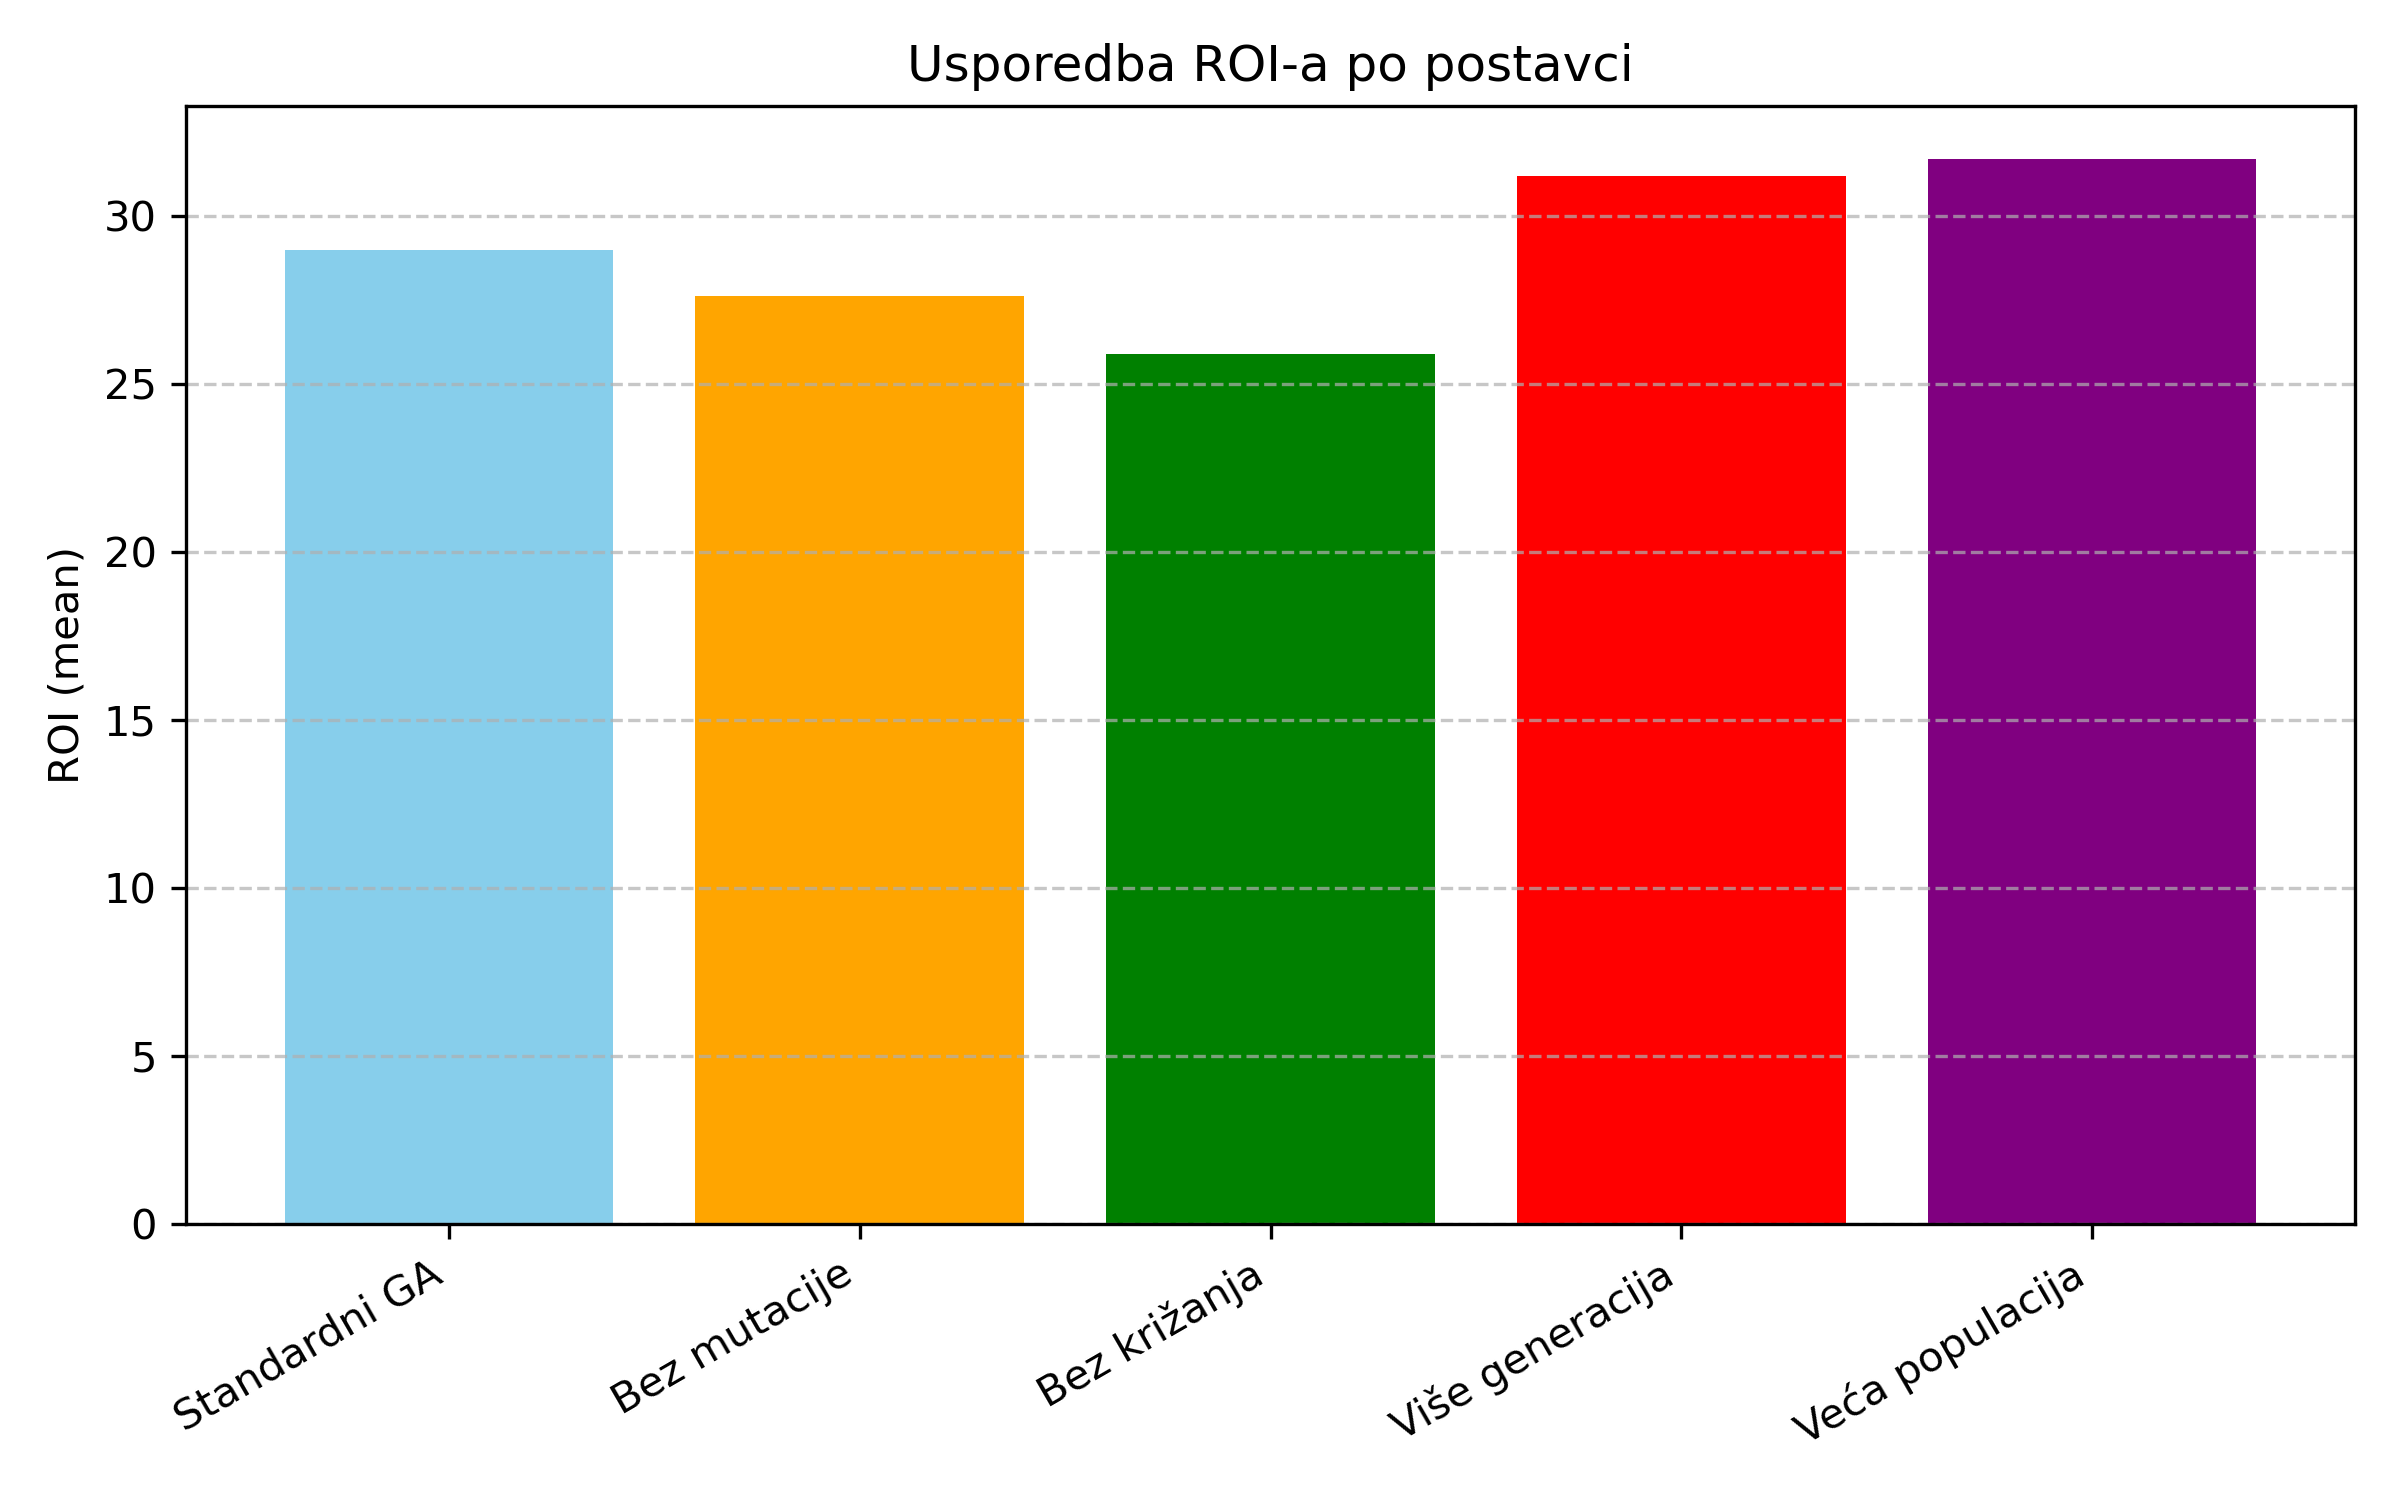
\includegraphics[width=\textwidth]{slike/ga_usporedba_roi.png}
        \caption{Usporedba prosječnog ROI-a za različite konfiguracije GA.}
        \label{fig:ga_roi}
    \end{subfigure}
    \hfill
    \begin{subfigure}[b]{0.48\textwidth}
        \centering
        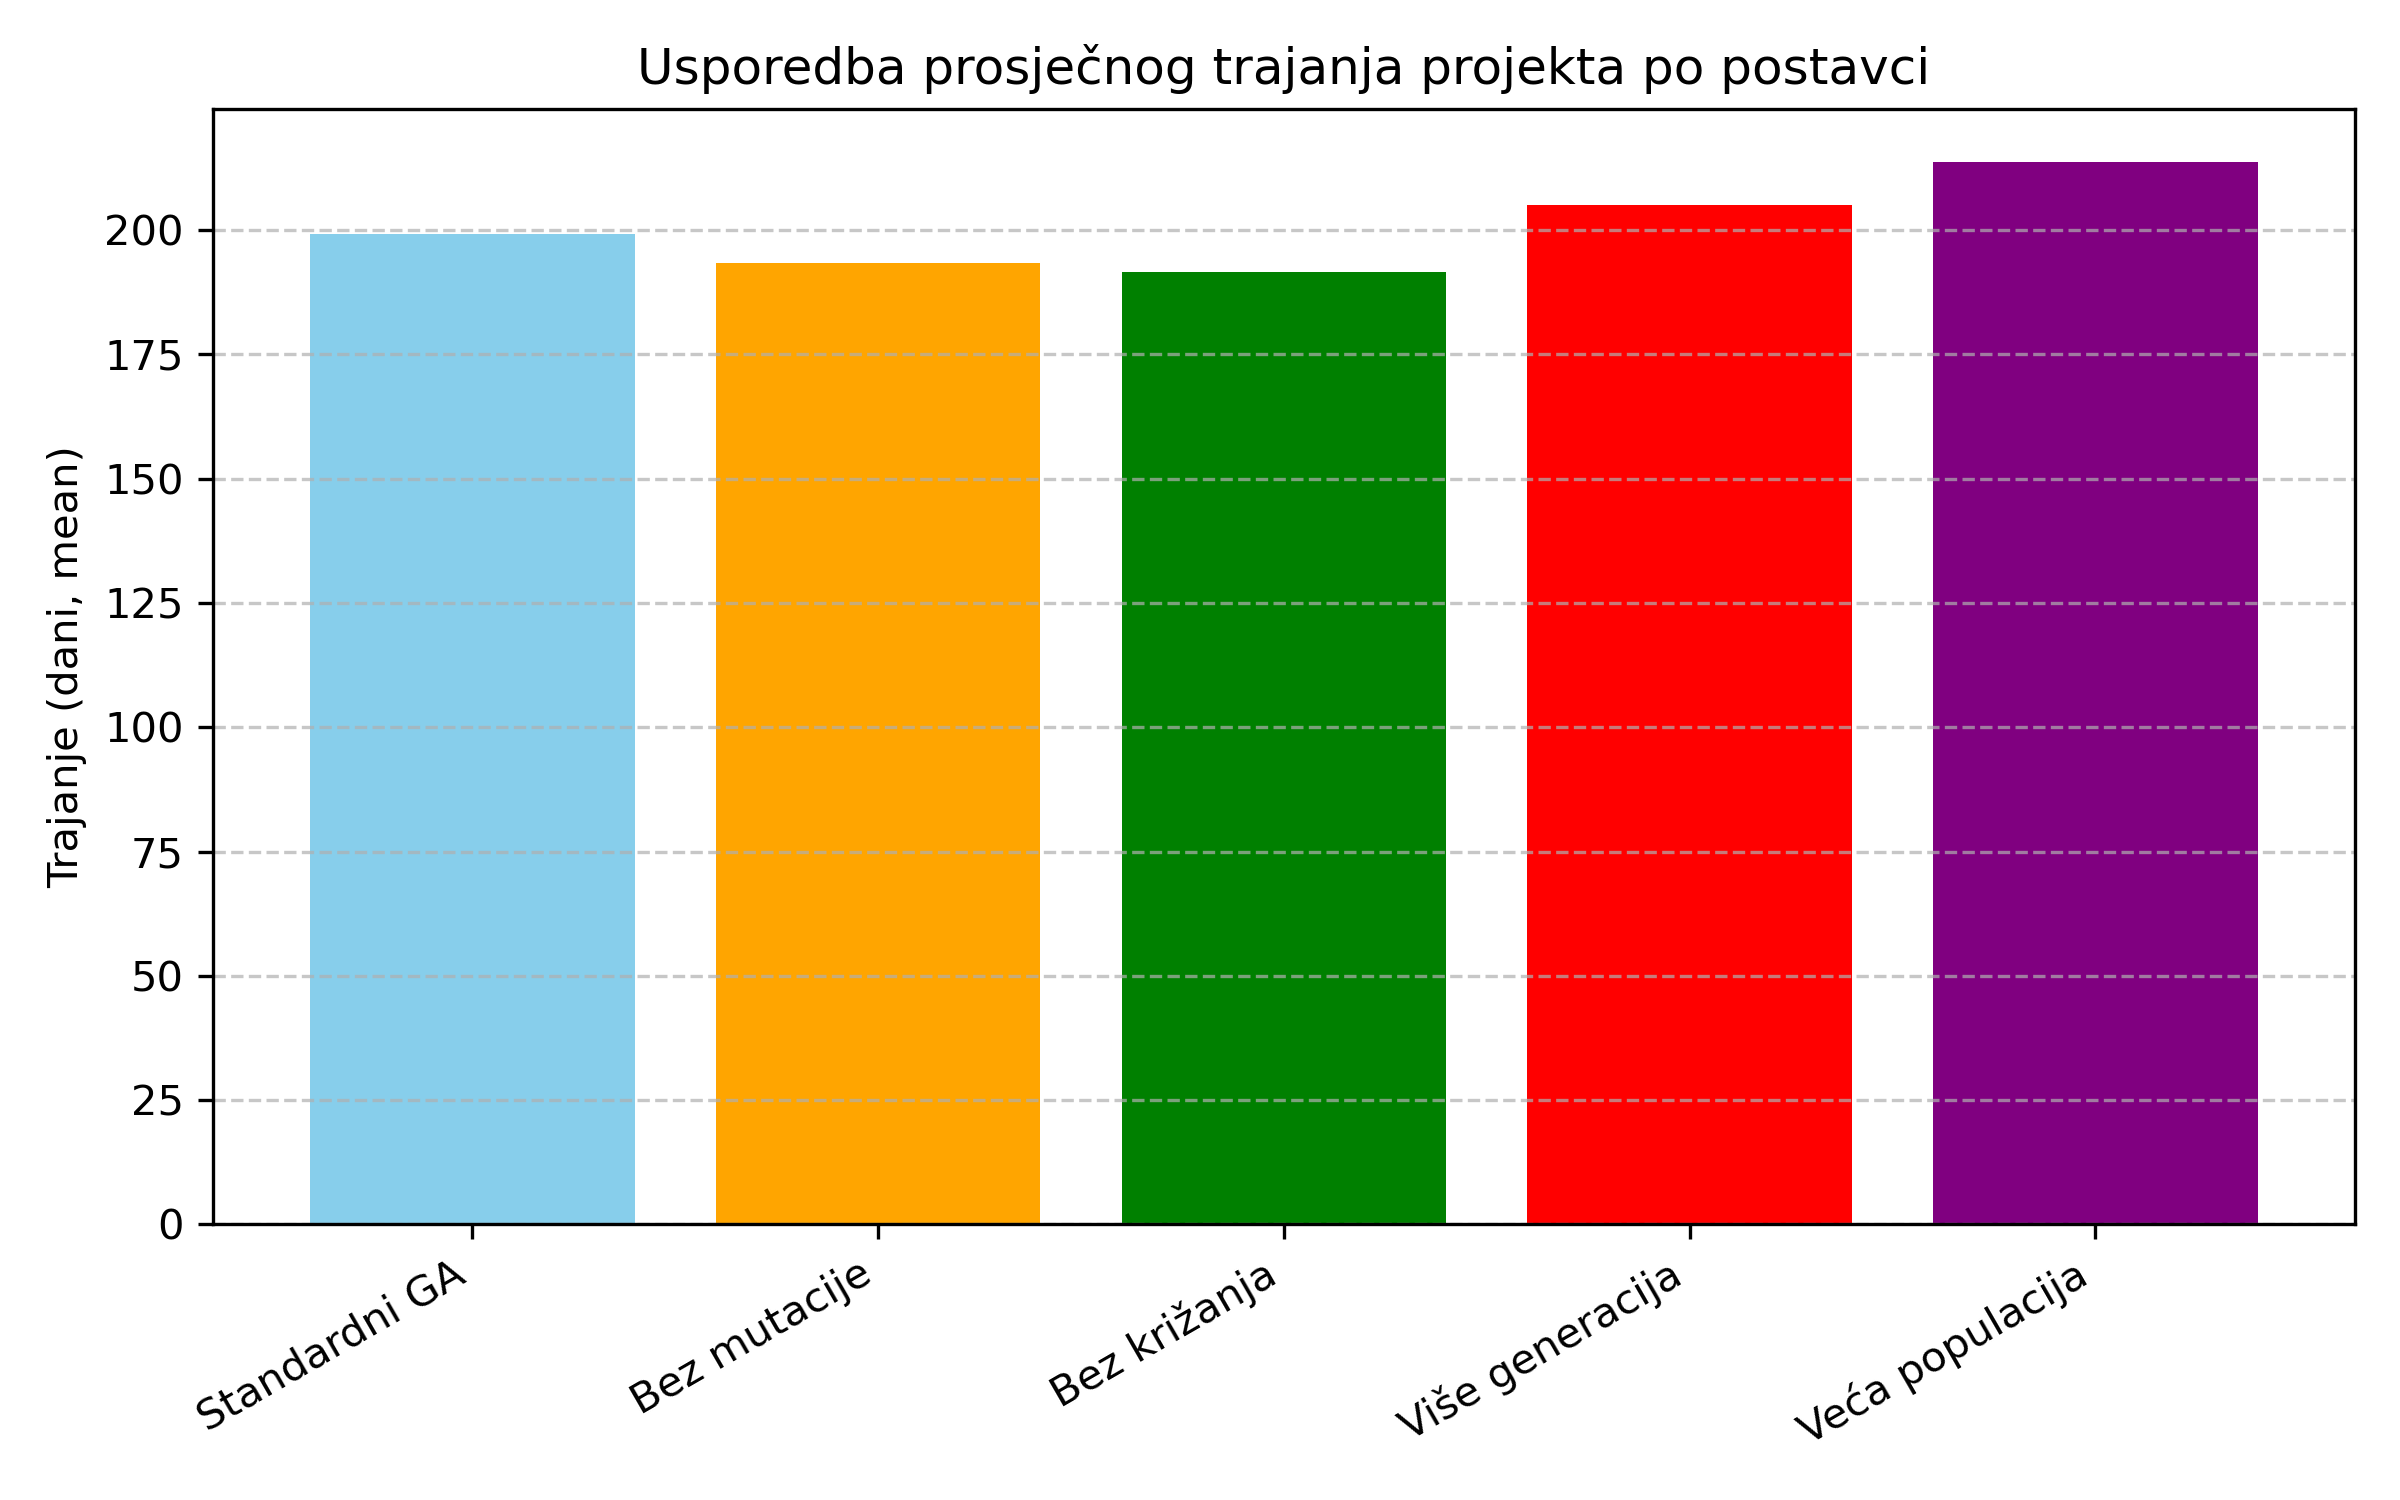
\includegraphics[width=\textwidth]{slike/ga_usporedba_trajanje.png}
        \caption{Usporedba prosječnog trajanja projekta za različite konfiguracije GA.}
        \label{fig:ga_trajanje}
    \end{subfigure}
    \caption{Grafički prikaz rezultata ablacijske studije za genetski algoritam.}
    \label{fig:ga_ablation}
\end{figure}

\textbf{Zaključak Eksperimenta 1:}  
Na temelju empirijskih rezultata, konfiguracija \emph{Veća populacija} odabrana je kao ``šampionska''. Njezini parametri (\texttt{POP\_SIZE = 200}, \texttt{NGEN = 40}, \texttt{CX\_PB = 0.7}, \texttt{MUT\_PB = 0.2}) koristit će se u svim daljnjim eksperimentima koji uključuju genetski algoritam, kako bi se osigurala njihova maksimalna učinkovitost i omogućila pravedna usporedba.

\subsection{Eksperiment 2: Usporedna analiza optimizacijskih modela}

Na slici \ref{fig:tok_eksperimenta} prikazan je dijagram toka izvođenja eksperimenta. 
\begin{figure}[]
    \centering
    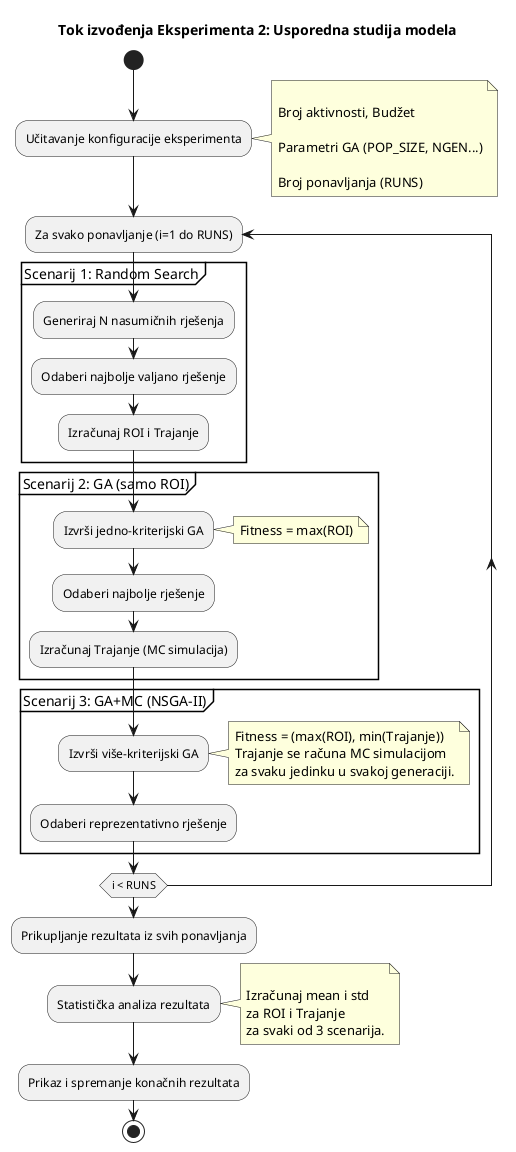
\includegraphics[width=0.75\textwidth]{slike/tok_eksperimenta2.png}
    \caption{Dijagram toka izvođenja eksperimenta}
    \label{fig:tok_eksperimenta}
\end{figure}

Nakon što je u Eksperimentu 1 provedena kalibracija i odabrana "šampionska" konfiguracija genetskog algoritma, u drugoj fazi istraživanja pristupilo se ključnoj usporednoj analizi triju razvijenih modela.

\subsubsection{Metodologija}
Cilj ovog eksperimenta bio je kvantitativno i kvalitativno usporediti performanse, kvalitetu i stabilnost rješenja dobivenih pomoću tri različita optimizacijska scenarija. Eksperimenti su provedeni prema planu definiranom u Tablici \ref{tab:plan_eksperimenata}. Svaka konfiguracija iz plana testirana je 10 puta (RUNS=10) radi osiguravanja statističke robusnosti zaključaka. Genetski algoritmi (GA (samo ROI) i GA+MC (NSGA-II)) koristili su "šampionsku" konfiguraciju parametara (POP\_SIZE = 200, NGEN = 40, itd.) utvrđenu u prethodnom koraku, uz skaliranje parametra NGEN sukladno složenosti problema.

\begin{table}[h!]
    \centering
    \resizebox{\textwidth}{!}{
    \begin{tabular}{|l|l|l|l|l|}
        \hline
        \textbf{Eksperiment} & \textbf{NUM\_ACTIVITIES} & \textbf{BUDGET} & \textbf{Pripada seriji} & \textbf{Napomena} \\
        \hline
        A1 & 10 & 1000 & A & Osnovna složenost \\
        \hline
        A2 / B2 & 50 & 2500 & A, B & Centralni / Referentni eksperiment \\
        \hline
        A3 & 100 & 5000 & A & Visoka složenost \\
        \hline
        B1 & 50 & 1500 & B & Restriktivan budžet \\
        \hline
        B3 & 50 & 4000 & B & Labav budžet \\
        \hline
    \end{tabular}
}
    \caption{Plan naprednih eksperimenata}
    \label{tab:plan_eksperimenata}
\end{table}

\subsubsection{Rezultati}
Svi rezultati dobiveni provođenjem Eksperimenta 2 sažeti su u Tablici \ref{tab:rezultati}. Ova tablica predstavlja temelj za daljnju diskusiju i donošenje zaključaka.

\begin{table}[h!]
    \centering
    \resizebox{\textwidth}{!}{
    \begin{tabular}{|l|l|l|l|l|l|}
        \hline
        \textbf{Eksperiment} & \textbf{Scenarij} & \textbf{ROI\_mean} & \textbf{ROI\_std} & \textbf{Trajanje\_mean} & \textbf{Trajanje\_std} \\
        \hline
        A1\_Osnovni & Random Search (MC) & 17.140 & 3.55e-15 & 144.15 & 10.911 \\
        \hline
        A1\_Osnovni & GA (samo ROI) & 17.140 & 3.55e-15 & 143.10 & 1.239 \\
        \hline
        A1\_Osnovni & GA+MC (NSGA-II) & 17.140 & 3.55e-15 & 142.00 & 0.372 \\
        \hline
        A2\_Srednji & Random Search (MC) & 40.108 & 0.703 & 341.02 & 9.405 \\
        \hline
        A2\_Srednji & GA (samo ROI) & 46.125 & 0.412 & 363.63 & 7.843 \\
        \hline
        A2\_Srednji & GA+MC (NSGA-II) & 44.099 & 0.980 & 319.21 & 13.171 \\
        \hline
        A3\_Slozeni & Random Search (MC) & 95.835 & 1.468 & 715.60 & 10.451 \\
        \hline
        A3\_Slozeni & GA (samo ROI) & 114.224 & 0.891 & 792.30 & 11.933 \\
        \hline
        A3\_Slozeni & GA+MC (NSGA-II) & 109.095 & 2.008 & 681.56 & 21.733 \\
        \hline
        B1\_Restriktivan & Random Search (MC) & 24.120 & 1.846 & 197.62 & 20.181 \\
        \hline
        B1\_Restriktivan & GA (samo ROI) & 37.976 & 0.567 & 253.56 & 12.386 \\
        \hline
        B1\_Restriktivan & GA+MC (NSGA-II) & 17.711 & 17.728 & 50104.38 & 49894.619 \\
        \hline
        B3\_Labav & Random Search (MC) & 71.379 & 1.114 & 536.90 & 16.247 \\
        \hline
        B3\_Labav & GA (samo ROI) & 79.065 & 0.518 & 562.19 & 9.345 \\
        \hline
        B3\_Labav & GA+MC (NSGA-II) & 76.949 & 0.487 & 526.61 & 10.602 \\
        \hline
    \end{tabular}
}
    \caption{Konačni rezultati usporedne analize optimizacijskih modela}
    \label{tab:rezultati}
\end{table}

\subsubsection{Diskusija rezultata}
Detaljna analiza rezultata provedena je kroz tri tematske cjeline, uz oslanjanje na vizualizacije generirane iz podataka u Tablici \ref{tab:rezultati}.

\textbf{Analiza Skalabilnosti (Serija A)}
\begin{figure}[H]
    \centering
    \begin{subfigure}[b]{0.48\textwidth}
        \centering
        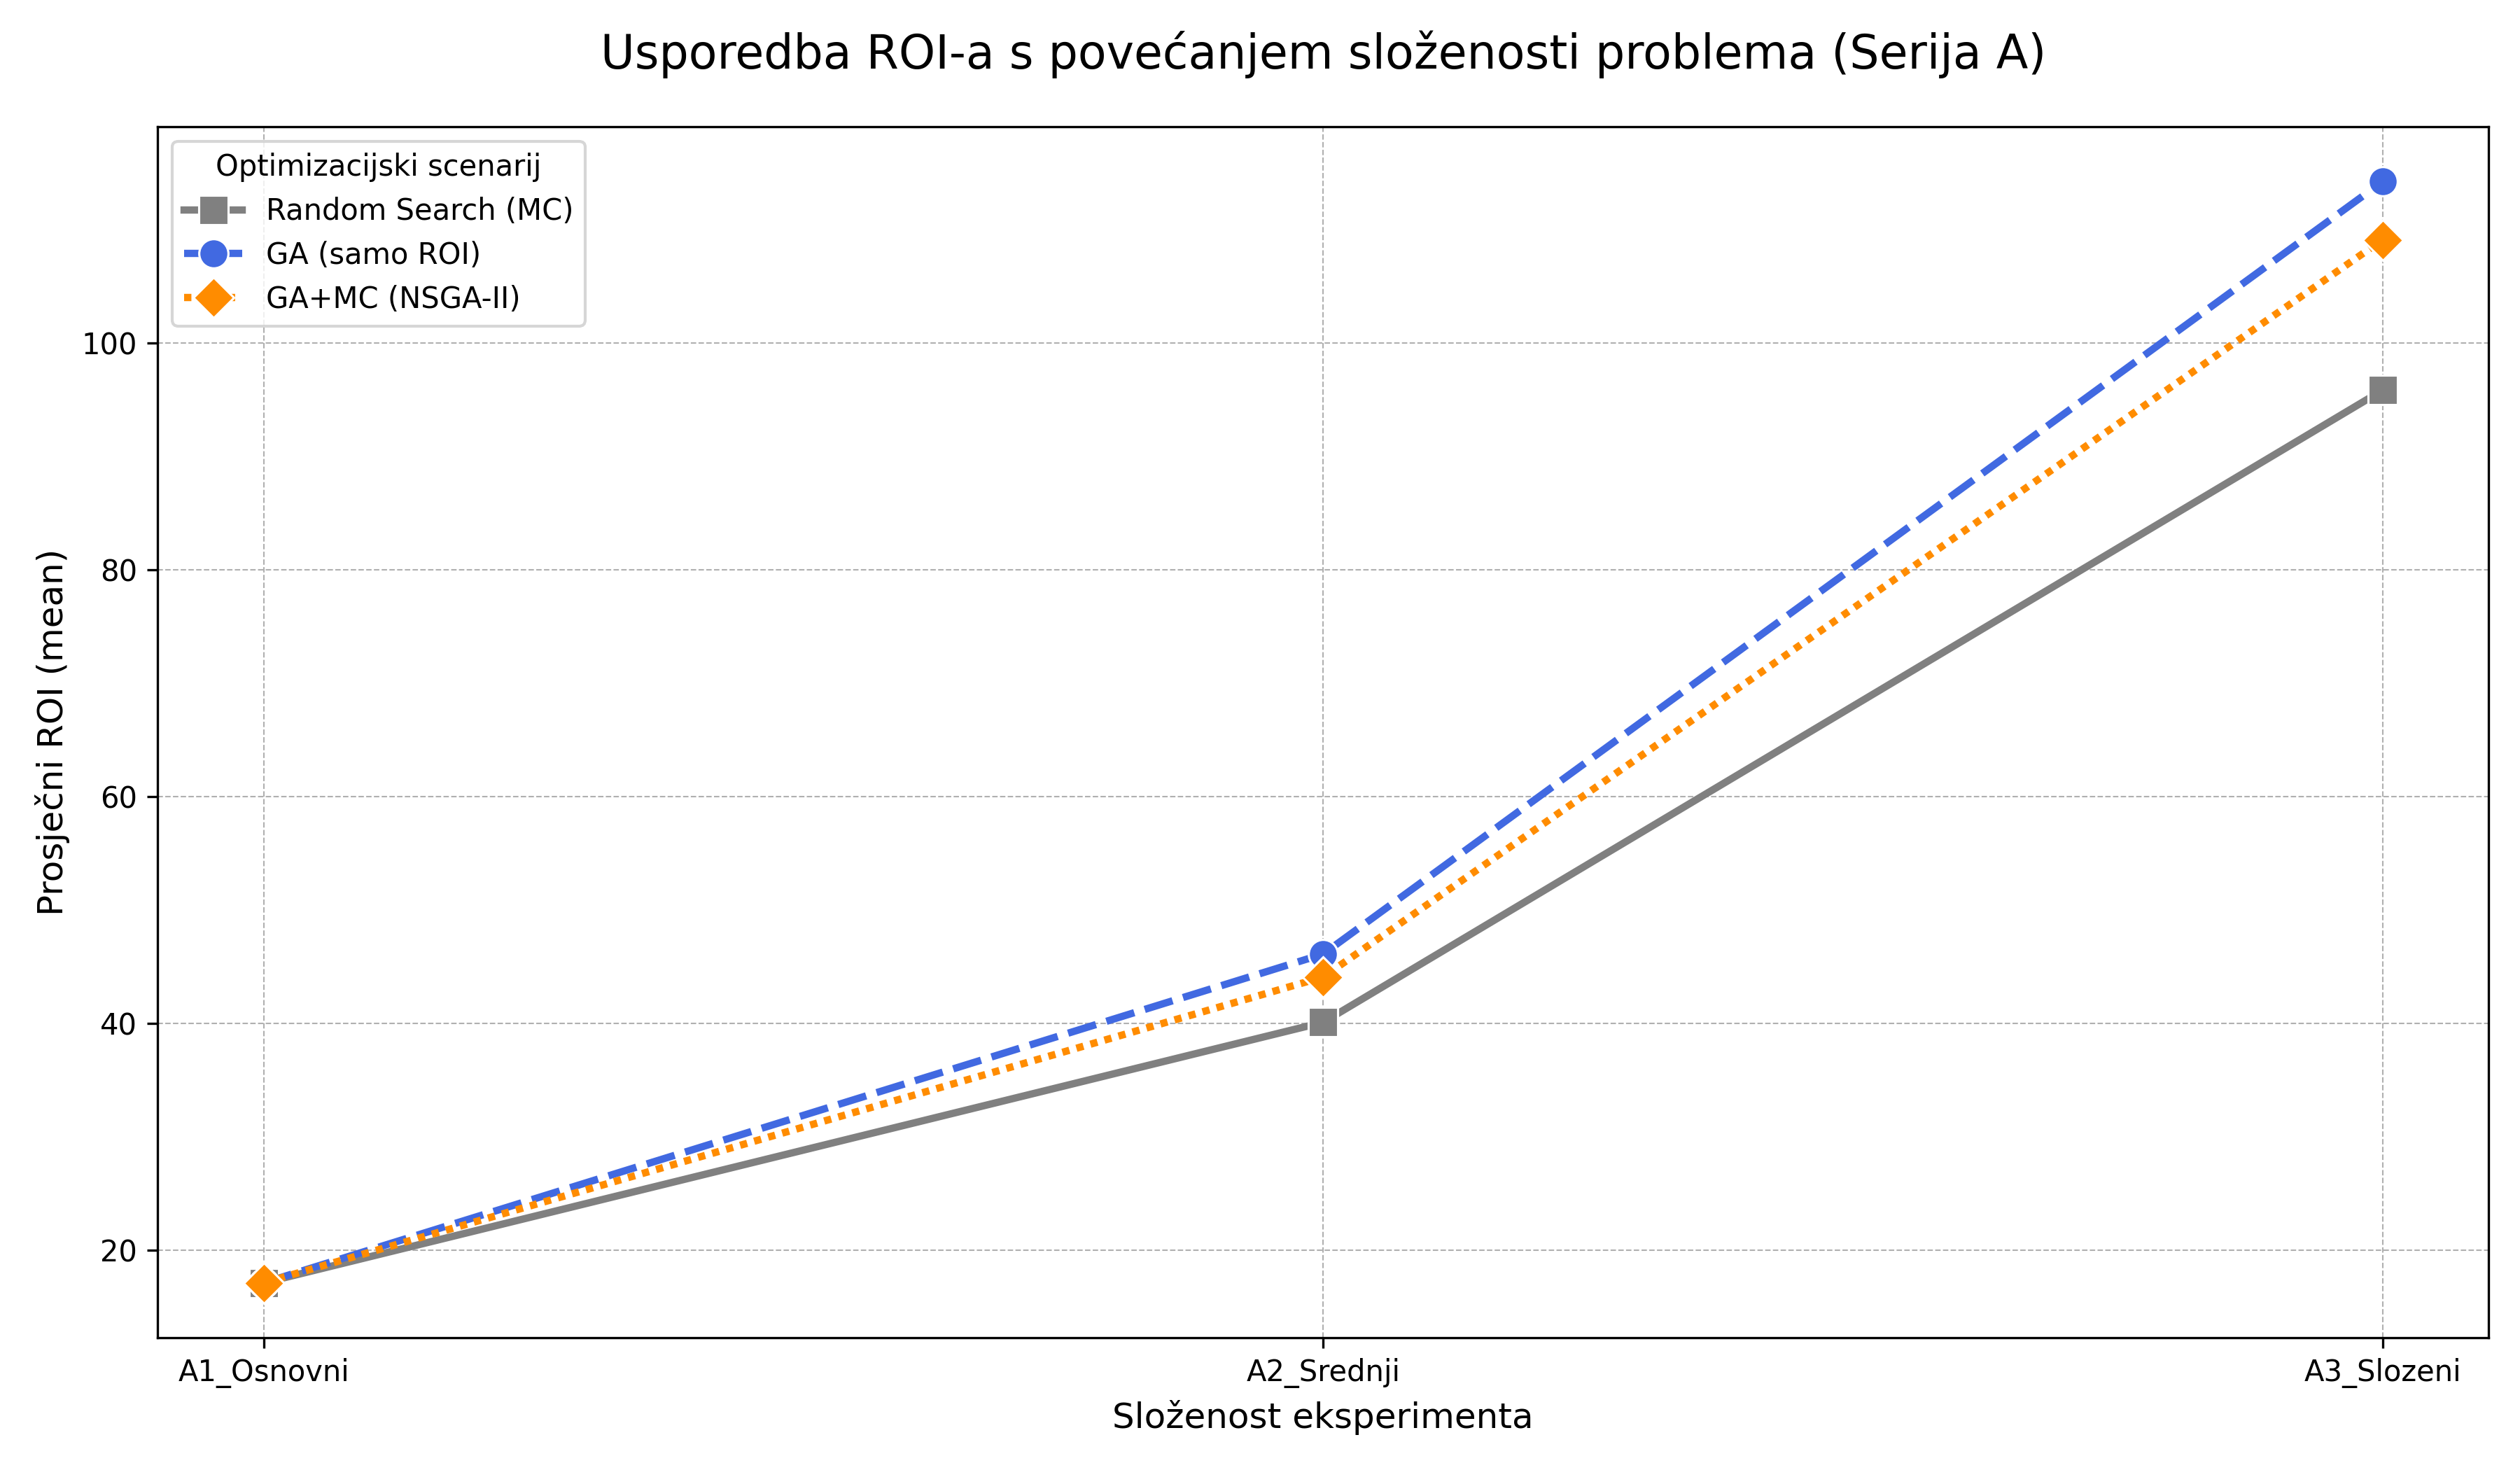
\includegraphics[width=\textwidth]{slike/grafikoni_final/A_skalabilnost_roi.png}
        \caption{Usporedba prosječnog ROI-a za tri različite konfiguracije.}
        \label{fig:a_ska_roi}
    \end{subfigure}
    \hfill
    \begin{subfigure}[b]{0.48\textwidth}
        \centering
        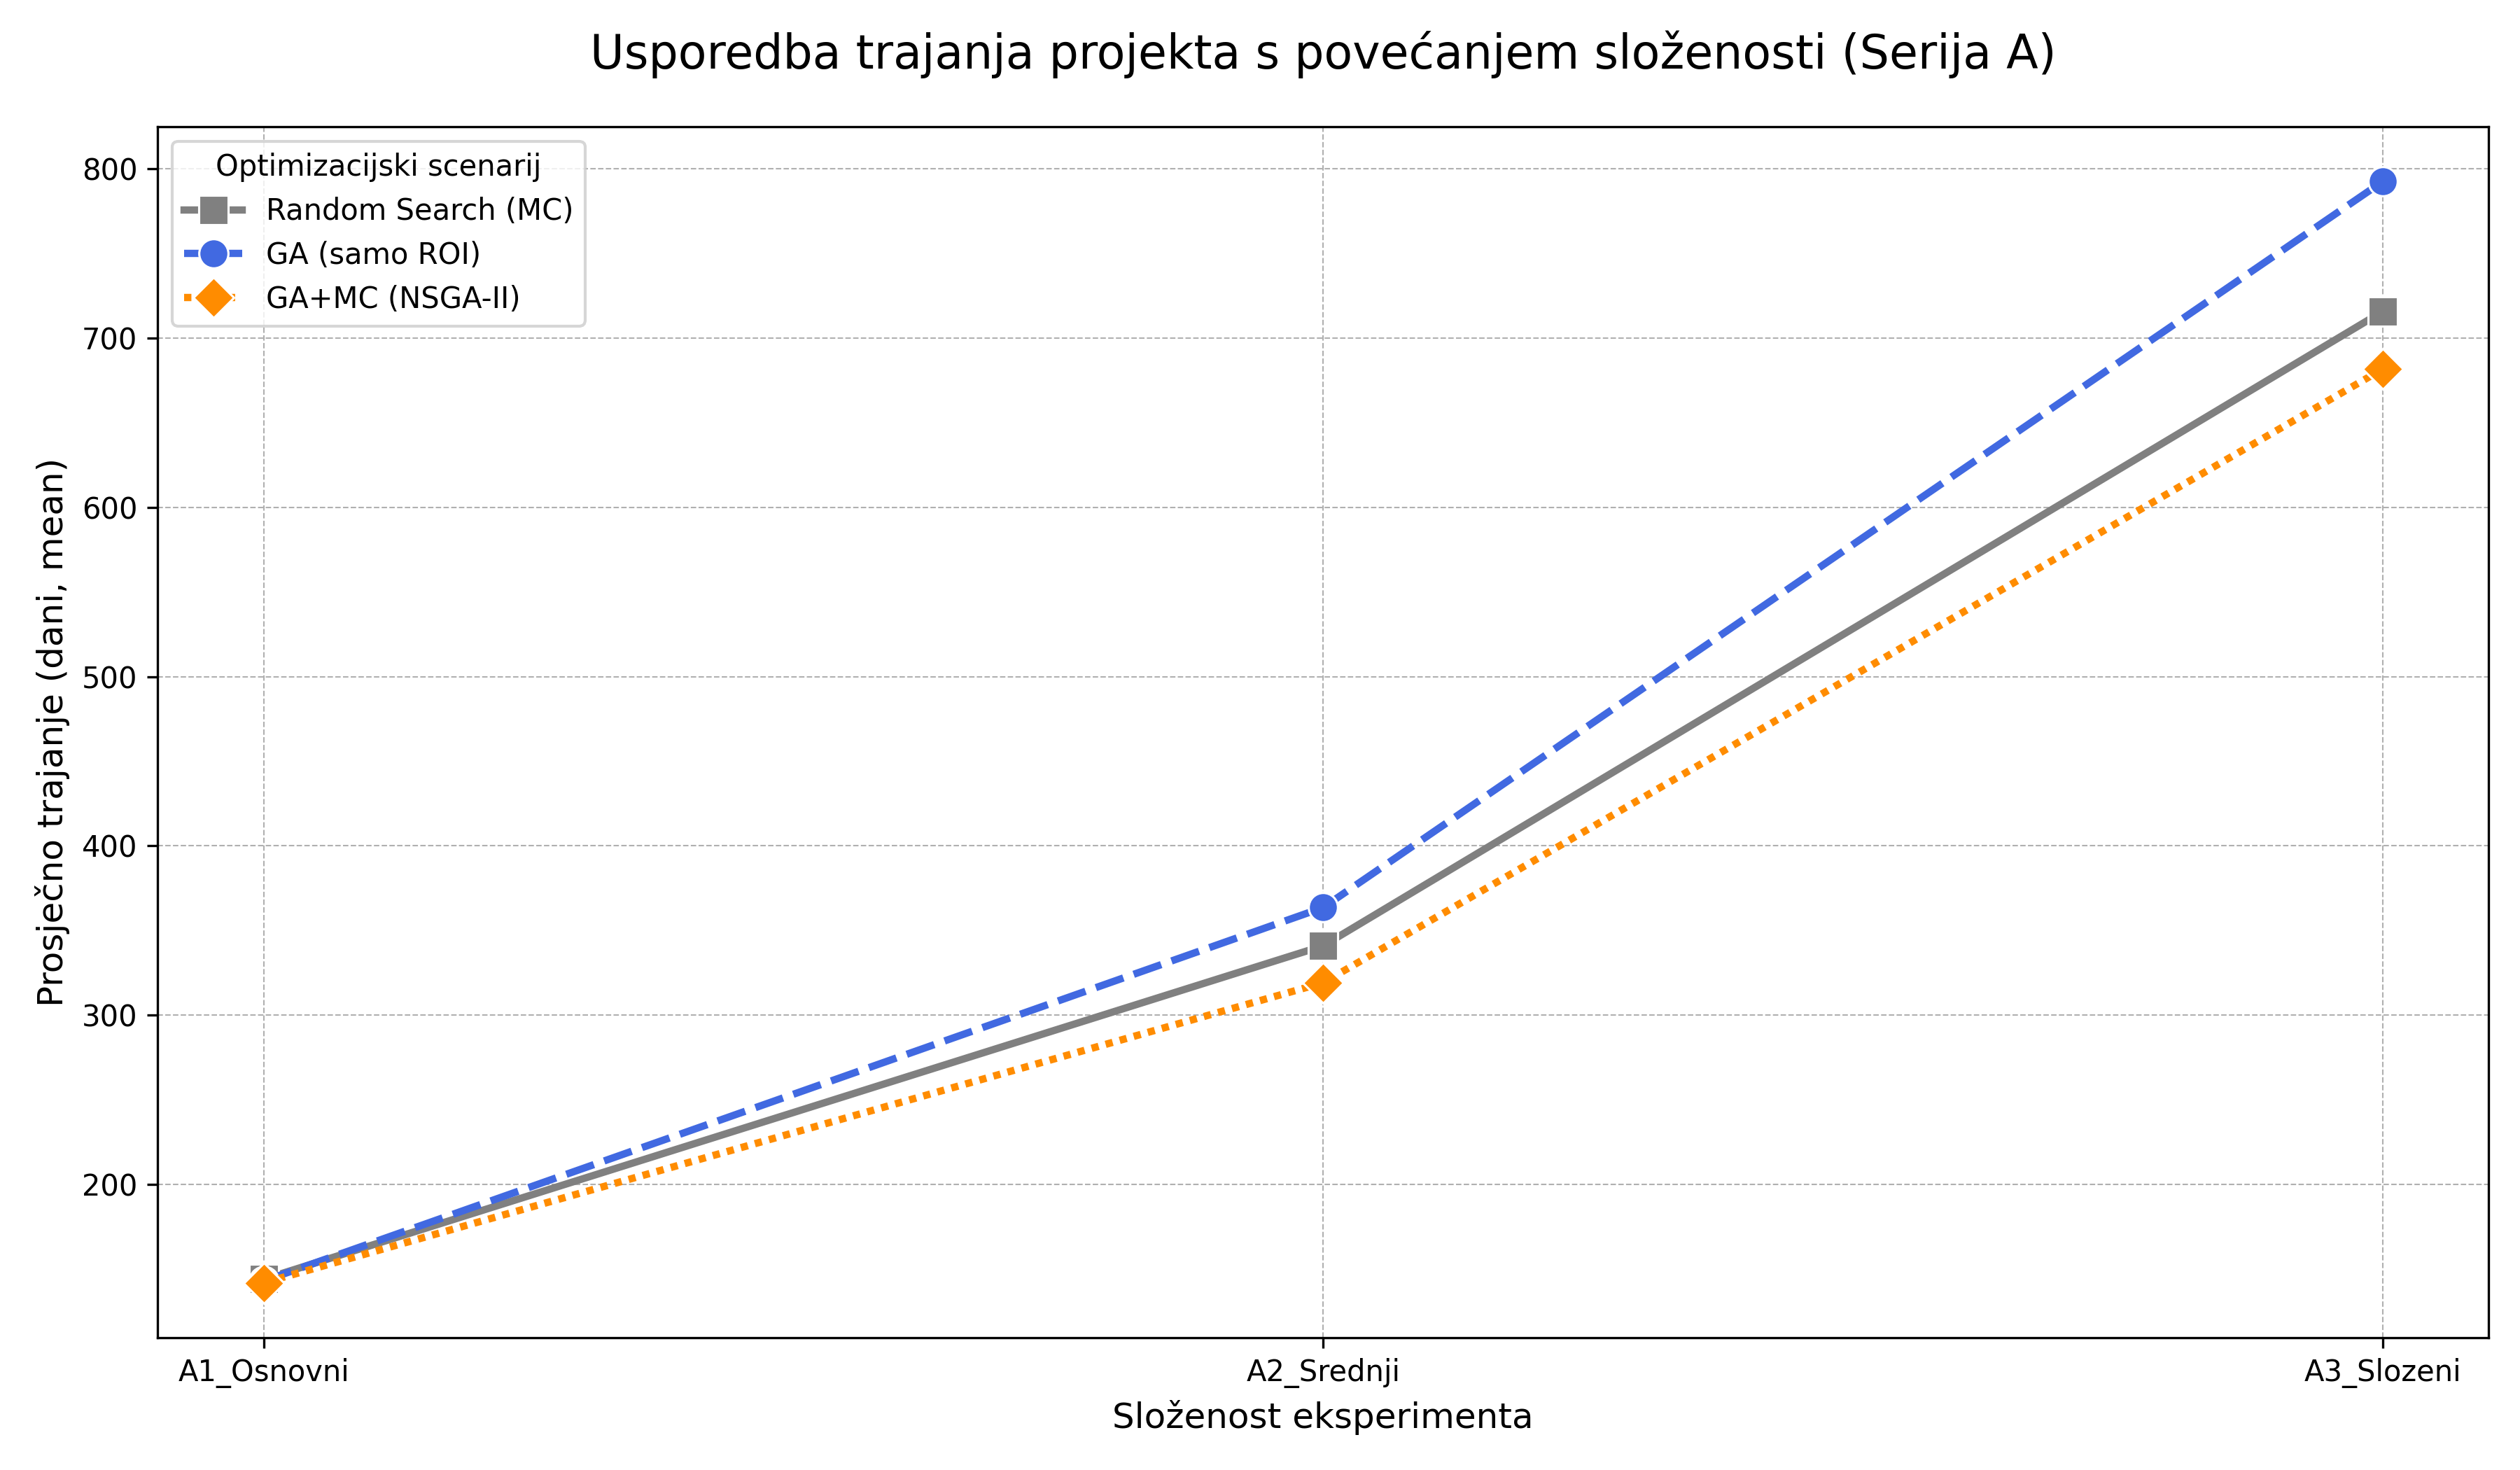
\includegraphics[width=\textwidth]{slike/grafikoni_final/A_skalabilnost_trajanje.png}
        \caption{Usporedba prosječnog trajanja projekta za tri različite konfiguracije.}
        \label{fig:a_ska_trajanje}
    \end{subfigure}
    \caption{Grafički prikaz rezultata usporednih  studija.}
    \label{fig:a_skalabilnost}
\end{figure}

Kao što je vidljivo na grafikonima \ref{fig:a_ska_roi} i \ref{fig:a_ska_trajanje}, porast složenosti problema s 10 na 100 aktivnosti drastično utječe na performanse modela. Dok su na osnovnom problemu (A1) sve metode pronašle isti financijski optimum, jaz u ROI\_mean vrijednostima eksponencijalno raste u korist genetskih algoritama. U eksperimentu A3, GA (samo ROI) ostvaruje prosječni ROI za preko 18 bodova viši od Random Search metode, što nedvojbeno potvrđuje hipotezu o nužnosti inteligentne pretrage (H1).
Istovremeno, analiza trajanja otkriva postojanje kompromisa. Hibridni model GA+MC (NSGA-II) konzistentno identificira rješenja sa značajno nižim prosječnim trajanjem. Na složenom problemu A3, ta razlika iznosi preko 110 dana u usporedbi s GA (samo ROI). Ovo potvrđuje hipotezu H2 – hibridni model uspješno upravlja rizikom, ali uz mjerljivu "cijenu" u vidu nešto nižeg maksimalnog ROI-a.

\textbf{Analiza Utjecaja Ograničenja (Serija B)}
\begin{figure}[]
    \centering
    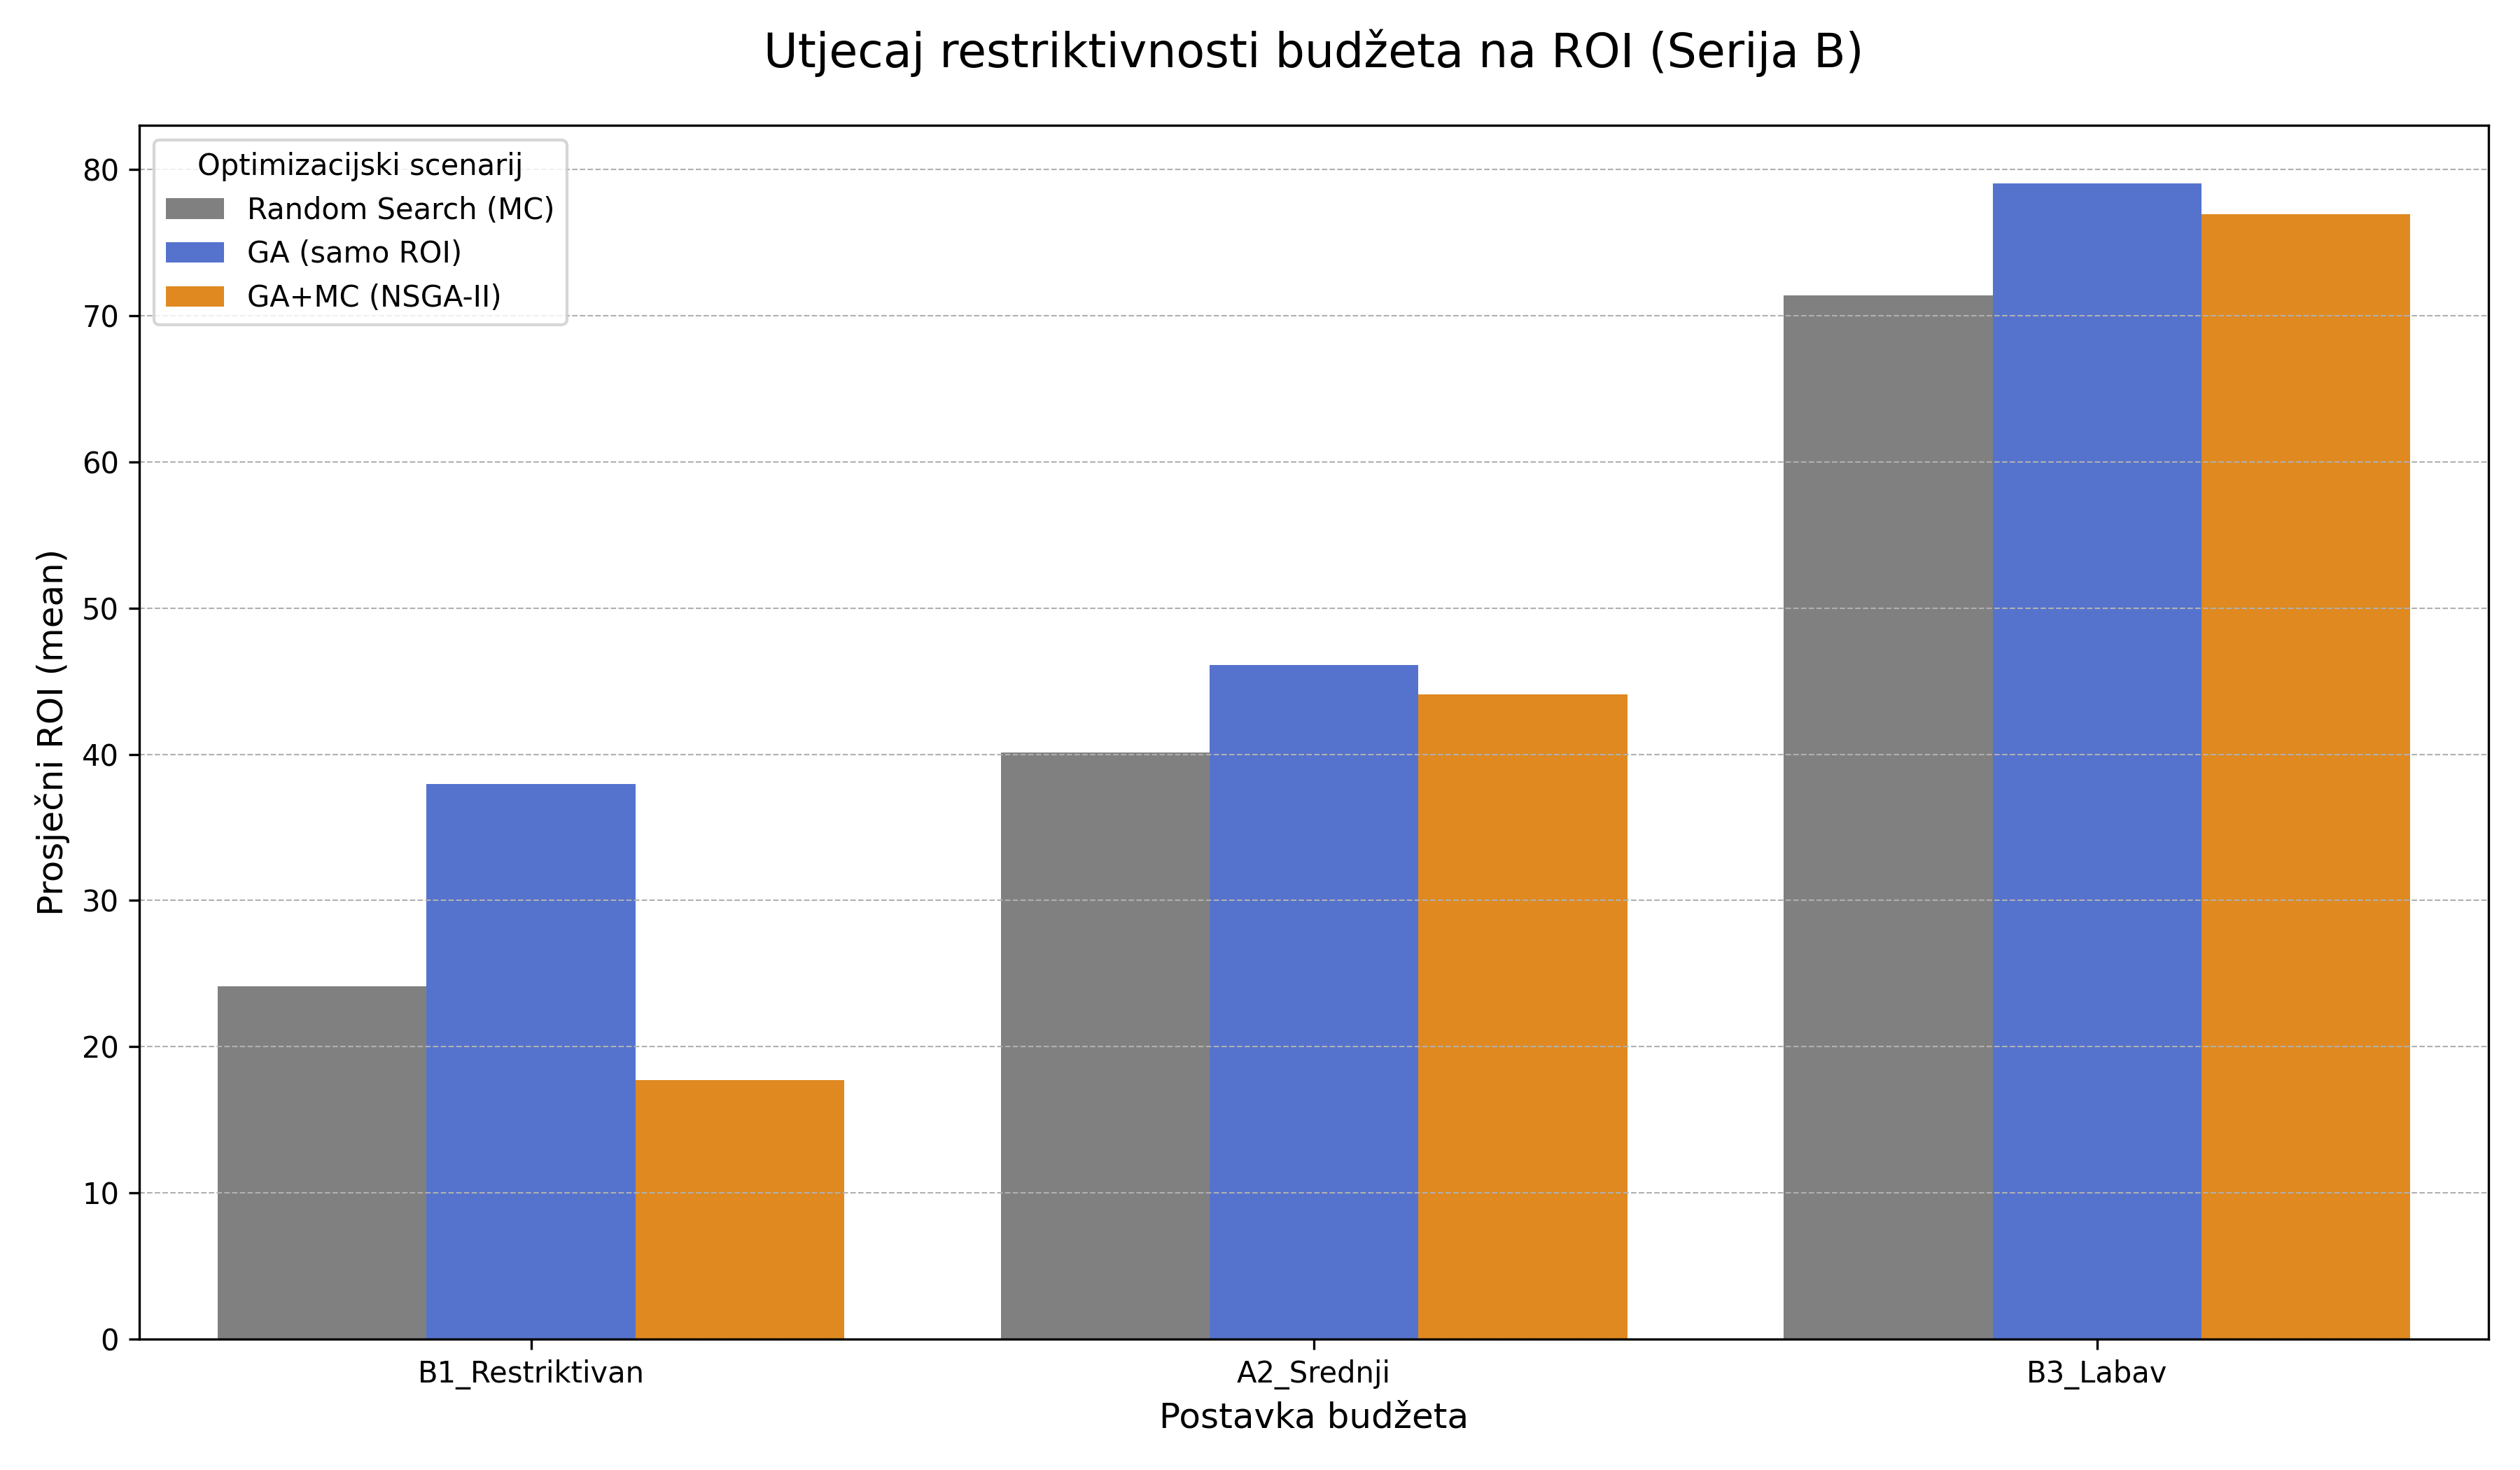
\includegraphics[width=0.75\textwidth]{slike/grafikoni_final/B_budzet_roi.png}
    \caption{Budžet}
    \label{fig:budzet_roi}
\end{figure}

Grafikon \ref{fig:budzet_roi} ilustrira ponašanje modela pod različitim proračunskim pritiskom. Najvažniji nalaz dolazi iz eksperimenta s restriktivnim budžetom (B1). U tim uvjetima, GA+MC (NSGA-II) pokazuje iznimnu krhkost, ne uspijevajući pronaći valjano rješenje u 50\% pokretanja, što rezultira katastrofalnim prosječnim performansama (Tablica \ref{tab:rezultati}, redak 11). S druge strane, jednostavniji GA (samo ROI) pokazuje se vrlo robusnim, uspješno pronalazeći visokoprofitabilna rješenja čak i u vrlo ograničenom prostoru. Ovo ukazuje da složenost više-kriterijske pretrage može biti nedostatak u ekstremno suženim prostorima rješenja.
U uvjetima labavog budžeta (B3), svi modeli rade očekivano dobro, a razlike među njima se smanjuju, potvrđujući hipotezu H3.

\textbf{Analiza Stabilnosti i Pouzdanosti}
\begin{figure}[H]
    \centering
    \begin{subfigure}[b]{0.48\textwidth}
        \centering
        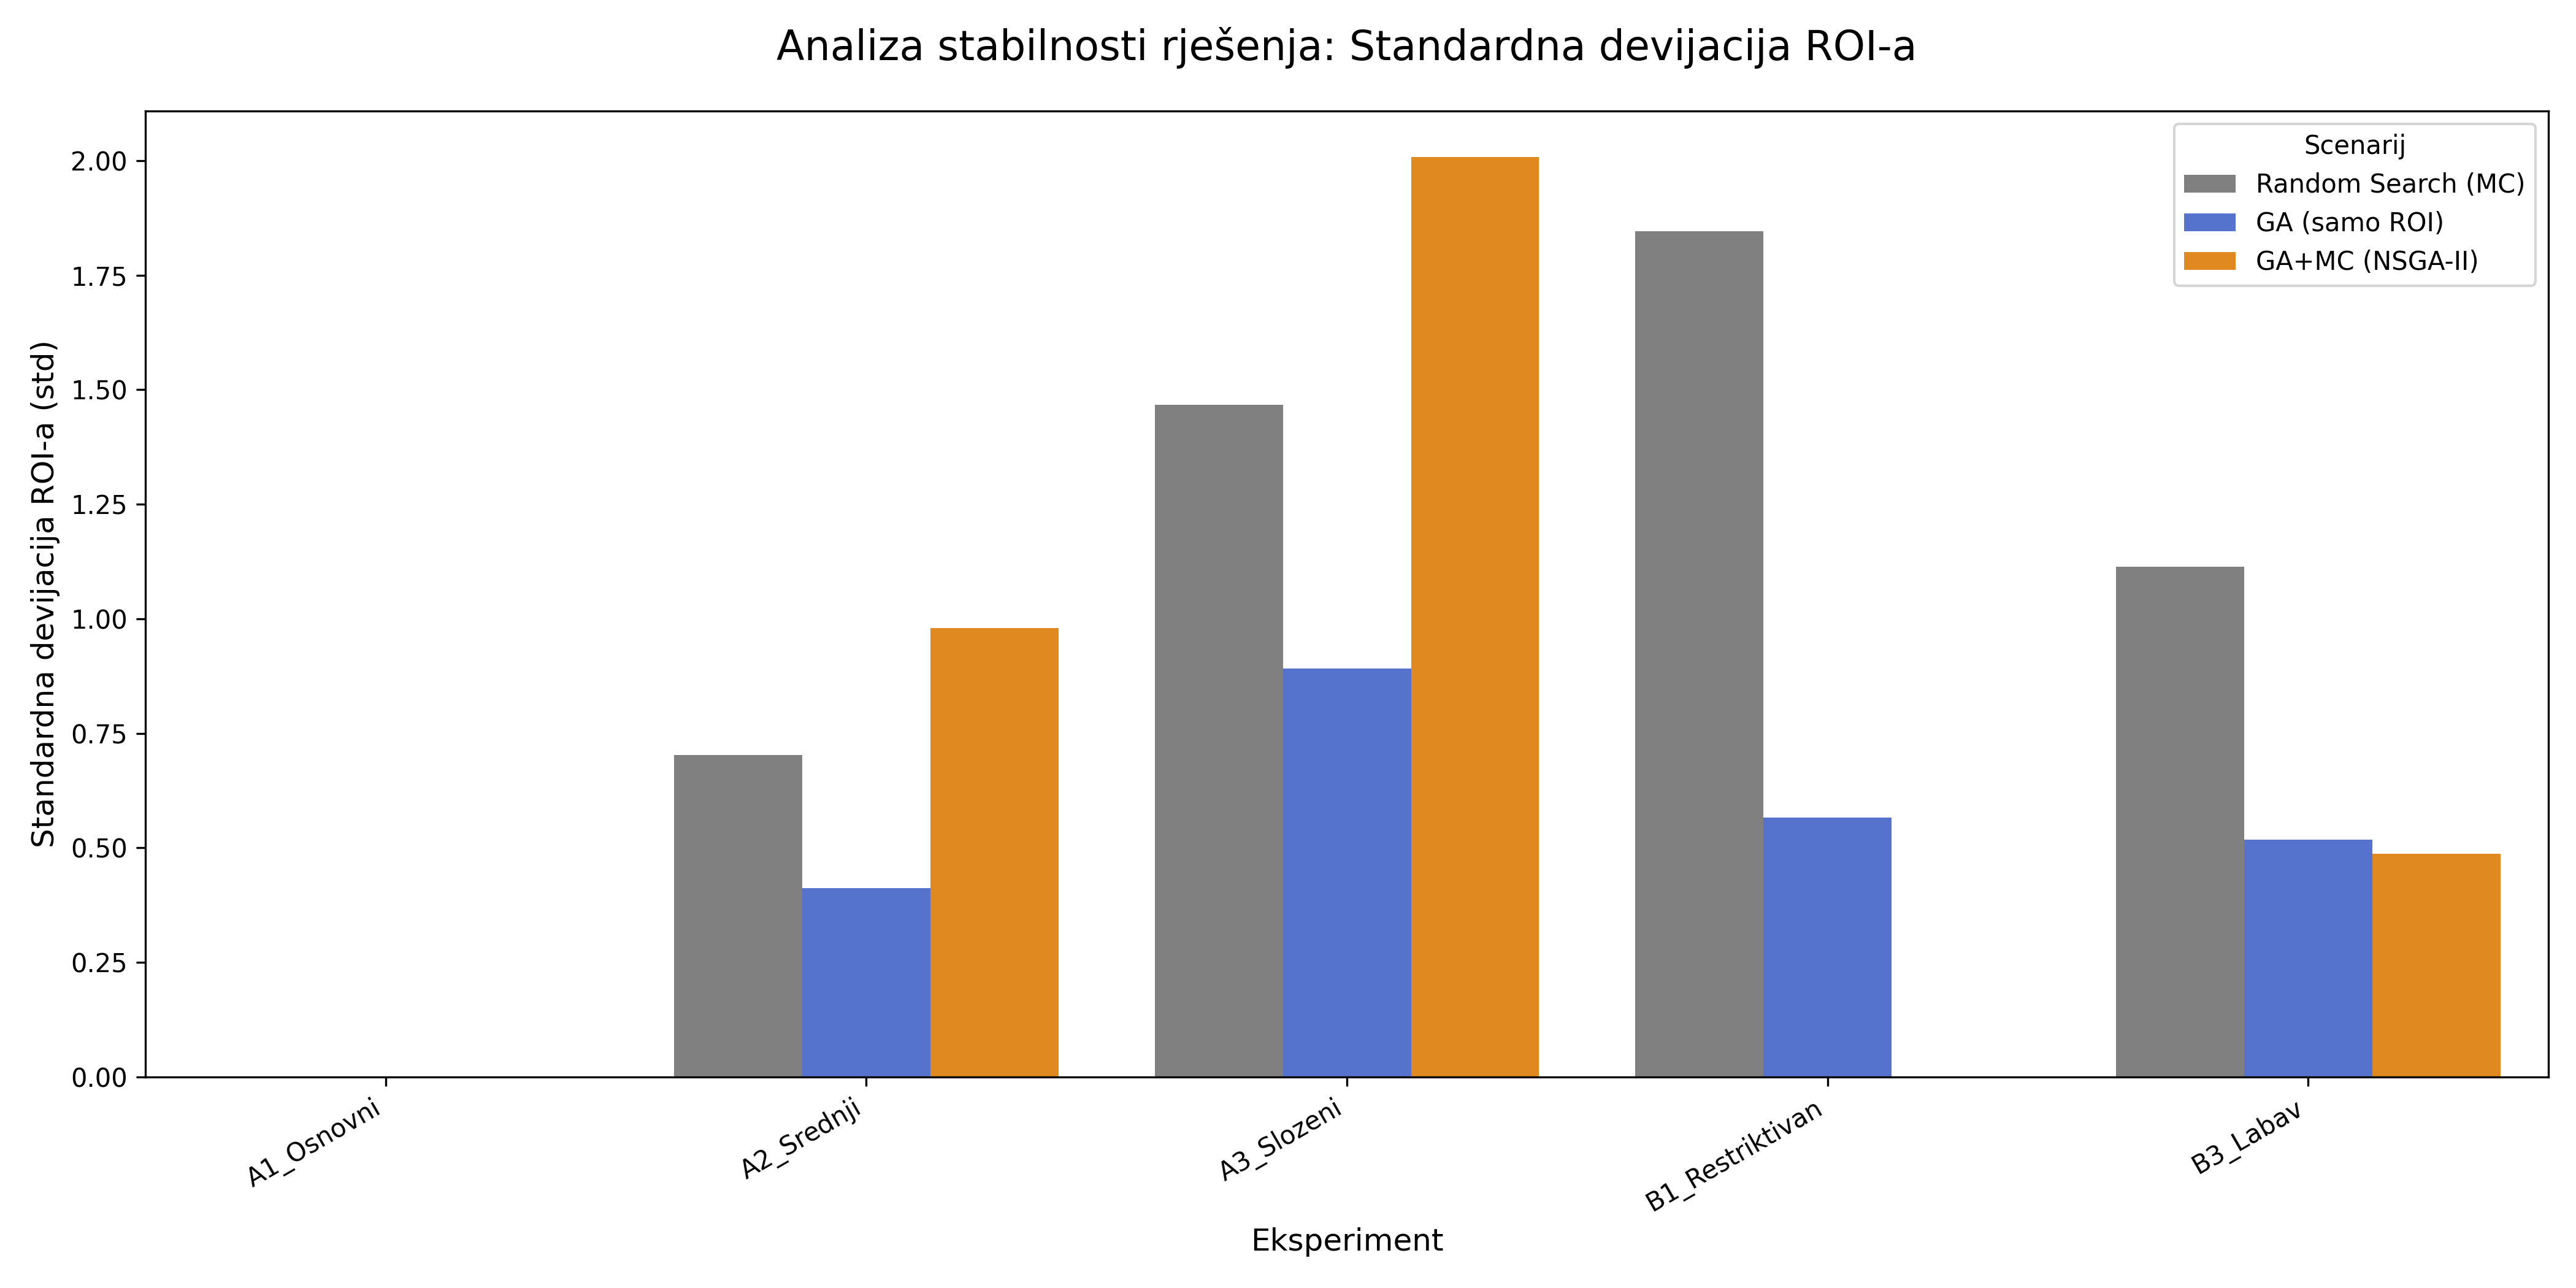
\includegraphics[width=\textwidth]{slike/grafikoni_final/C_stabilnost_roi.png}
        \caption{Stabilnost ROI-a za tri različite konfiguracije.}
        \label{fig:stab_roi}
    \end{subfigure}
    \hfill
    \begin{subfigure}[b]{0.48\textwidth}
        \centering
        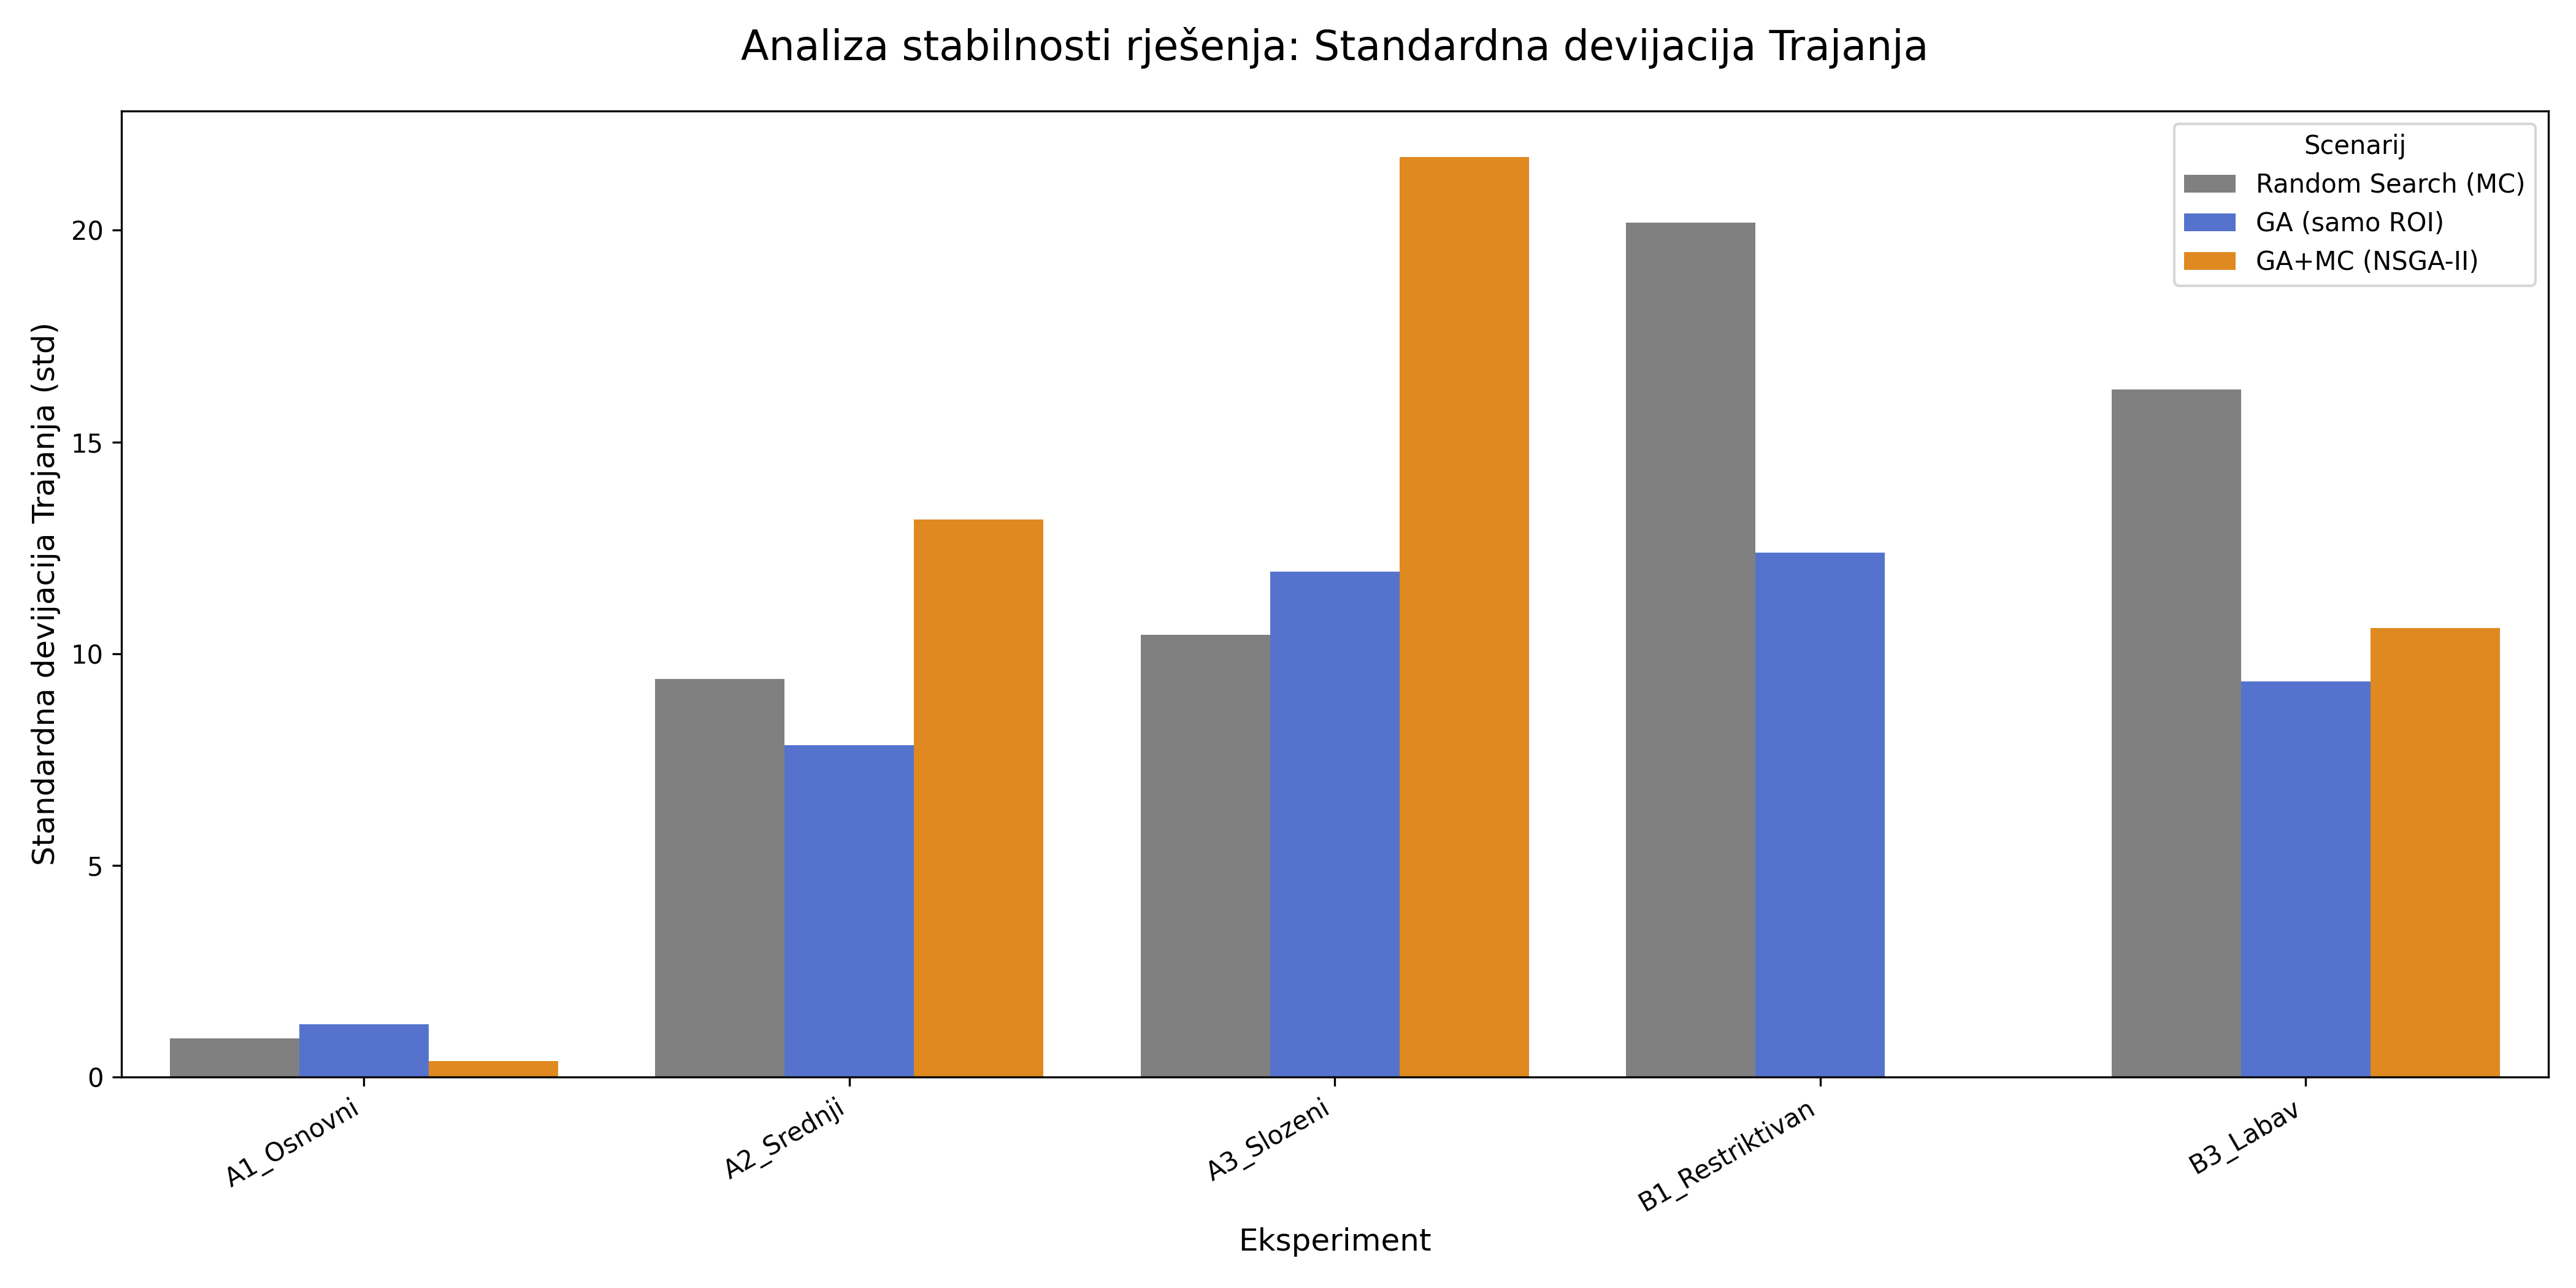
\includegraphics[width=\textwidth]{slike/grafikoni_final/C_stabilnost_trajanje.png}
        \caption{Stabilnost trajanja projekta za tri različite konfiguracije.}
        \label{fig:stab_trajanje}
    \end{subfigure}
    \caption{Grafički prikaz rezultata usporednih  studija.}
    \label{fig:a_skalabilnost}
\end{figure}

Grafikoni \ref{fig:stab_roi} i \ref{fig:stab_trajanje} prikazuju standardnu devijaciju kao mjeru konzistentnosti. Izvan scenarija B1 gdje je doživio neuspjeh, GA+MC (NSGA-II) model pokazuje usporedivu ili nižu devijaciju trajanja u odnosu na klasični GA. To implicira da rješenja koja nudi nisu samo u prosjeku brža, već su i pouzdanija, odnosno njihovo procijenjeno trajanje manje varira. Ova predvidljivost je od iznimne važnosti za praktično upravljanje projektima.

\subsubsection{Sinteza glavnih zaključaka eksperimenata}
\begin{itemize}
    \item \textbf{Random Search (MC):} Koristan kao početna točka i za jednostavne probleme, ali potpuno neadekvatan kao ozbiljan optimizacijski alat za probleme realne veličine i složenosti.
    \item \textbf{GA (samo ROI):} Izuzetno snažan i robustan "profitni maksimizator". Najbolji je izbor u situacijama gdje je financijska dobit jedini i isključivi kriterij, te pokazuje veliku otpornost u uvjetima strogih ograničenja.
    \item \textbf{GA+MC (NSGA-II):} Sofisticirani "upravitelj rizikom". Njegova najveća vrijednost je u pružanju strateških opcija koje balansiraju profit i rizik (trajanje). Superioran je u standardnim i složenim uvjetima, ali njegova složenost ga čini osjetljivim i nepouzdanim u okruženjima s ekstremno restriktivnim ograničenjima.
\end{itemize}
Konačan izbor modela stoga ovisi o strateškim prioritetima projektnog ureda. Za maksimalan profit, klasični GA je pobjednik. Za uravnoteženo i rizikom informirano donošenje odluka, hibridni GA+MC je superioran, uz nužan oprez pri primjeni u vrlo ograničenim uvjetima.
